% DISCELL -- RECOMB submission, main text.
% Build: ./build.sh  (builds main.pdf and supplement.pdf; cross-references via xr-hyper)
% Format: letter paper, 10 pt, 1-inch margins, two columns; separate title page (not counted);
% at most 10 pages of main text including floats; bibliography not counted.
\documentclass[letterpaper,10pt,twocolumn]{article}

\usepackage[letterpaper,margin=1in]{geometry}
\setlength{\columnsep}{0.25in}

\usepackage[numbers,sort&compress]{natbib}
\usepackage{amsmath,amssymb,amsthm,bm,mathtools}
\usepackage{graphicx}
\usepackage{booktabs,multirow,array,longtable}
\usepackage{subcaption}
\usepackage{xcolor}
\usepackage{microtype}
\usepackage{enumitem}
\PassOptionsToPackage{hyphens}{url}
\usepackage{xr-hyper}   % must precede hyperref
\usepackage[colorlinks=true,linkcolor=blue!60!black,citecolor=blue!60!black,urlcolor=blue!60!black]{hyperref}
\usepackage{pdfpages}
\usepackage[capitalise]{cleveref}
% short reference names to save space (author, 2026-10-01)
\crefname{figure}{Fig.}{Figs.}\Crefname{figure}{Fig.}{Figs.}
\crefname{table}{Table}{Tables}\Crefname{table}{Table}{Tables}
\crefname{section}{Sec.}{Secs.}\Crefname{section}{Sec.}{Secs.}
\crefname{equation}{Eq.}{Eqs.}\Crefname{equation}{Eq.}{Eqs.}
\renewcommand{\figurename}{Fig.}

% shared resources: one output location for the figure and table generators
\graphicspath{{../aistats/figures/}}
\newcommand{\tablesdir}{../aistats/tables/generated}
\renewcommand{\dbltopfraction}{0.95}
% ---------------------------------------------------------------------------
% Notation and editorial macros for the DISCELL manuscript (RECOMB copy of ../aistats/macros.tex)
% ---------------------------------------------------------------------------
\newcommand{\needsource}{\textcolor{red}{\textbf{[NEEDS A SOURCE]}}}
\newcommand{\todo}[1]{\textcolor{orange}{\textbf{[TODO: #1]}}}
\newcommand{\pending}[1]{\textcolor{violet}{\textbf{[PENDING RUNS: #1]}}}
% editorial flags and reading-order markers: no-ops in the RECOMB version
% (kept so that text copied from the AISTATS sources compiles; delete calls when editing)
\DeclareRobustCommand{\flag}[2]{\ignorespaces}
\DeclareRobustCommand{\readorder}[1]{\ignorespaces}
% code link placeholder (the clean repository comes later)
\newcommand{\codelink}{\textcolor{violet}{\texttt{[URL to be added]}}}

% vocabulary of the generated tables (shared by both manuscripts): RECOMB words (STYLE.md); ../aistats/macros.tex defines the AISTATS ones
\newcommand{\termSpill}{spill-over}
\newcommand{\TermSpill}{Spill-over}
\newcommand{\termSpillFrac}{spill-over fraction}
\newcommand{\TermSpillFrac}{Spill-over fraction}
\newcommand{\termReloc}{relocation}
\newcommand{\TermReloc}{Relocation}
\newcommand{\termInflux}{spill-over influx}
\newcommand{\TermInflux}{Spill-over influx}

% operators
\DeclareMathOperator{\sgop}{sg}
\newcommand{\sg}[1]{\sgop\!\left[#1\right]}
\DeclareMathOperator{\KL}{KL}
\DeclareMathOperator{\softmax}{softmax}
\DeclareMathOperator{\Mult}{Multinomial}
\DeclareMathOperator{\Pois}{Poisson}
\DeclareMathOperator{\CE}{CE}
\DeclareMathOperator{\diag}{diag}
\DeclareMathOperator{\logdet}{logdet}
\DeclareMathOperator{\embed}{embed}
\DeclareMathOperator{\onehot}{onehot}
\DeclareMathOperator{\GAT}{GATv2}
\DeclareMathOperator{\I}{I}
\DeclareMathOperator{\E}{\mathbb{E}}
\DeclareMathOperator{\Var}{Var}
\DeclareMathOperator{\corr}{corr}
\DeclareMathOperator{\NMI}{NMI}
\DeclareMathOperator{\simop}{sim}
\newcommand{\att}{\pi}   % attention weight, distinct from the loss weights alpha

% sets and fields
\newcommand{\R}{\mathbb{R}}
\newcommand{\Nat}{\mathbb{N}}
\newcommand{\N}{\mathcal{N}}
\newcommand{\simplex}[1]{\Delta^{#1}}
\newcommand{\nbr}[1]{\mathcal{N}_{#1}}

% vectors
\newcommand{\vx}{\mathbf{x}}
\newcommand{\vy}{\mathbf{y}}
\newcommand{\vz}{\mathbf{z}}
\newcommand{\vw}{\mathbf{w}}
\newcommand{\vc}{\mathbf{c}}
\newcommand{\vv}{\mathbf{v}}
\newcommand{\vu}{\mathbf{u}}
\newcommand{\vB}{\mathbf{B}}
\newcommand{\vI}{\mathbf{I}}
\newcommand{\vPhi}{\boldsymbol{\Phi}}
\newcommand{\vrho}{\boldsymbol{\rho}}
\newcommand{\rhobar}{\bar{\boldsymbol{\rho}}}
\newcommand{\vp}{\mathbf{p}}
\newcommand{\vmu}{\boldsymbol{\mu}}
\newcommand{\vsigma}{\boldsymbol{\sigma}}
\newcommand{\wbreve}{\breve{\mathbf{w}}}
\newcommand{\ybar}{\bar{\mathbf{y}}}
\newcommand{\Phibar}{\bar{\boldsymbol{\Phi}}}
\newcommand{\Sig}{\boldsymbol{\Sigma}}
\newcommand{\Sighat}{\hat{\boldsymbol{\Sigma}}}
\newcommand{\lbar}{\bar{\ell}}
\newcommand{\ephi}{e^{\Phi}}
\newcommand{\Ephi}{E_{\Phi}}
\newcommand{\dz}{d_z}
\newcommand{\dw}{d_w}
\newcommand{\dPhi}{d_{\Phi}}
\newcommand{\alphaz}{\alpha_z}
\newcommand{\alphaw}{\alpha_w}
\newcommand{\alphaa}{\alpha_a}
\newcommand{\mpsi}{m_{\psi}}
\newcommand{\Pen}{\mathrm{Pen}}
\newcommand{\Adv}{\mathrm{Adv}}
\newcommand{\dCE}{\Delta\!\CE}
\newcommand{\um}{\,\mu\text{m}}

\newtheorem{proposition}{Proposition}
\newtheorem{remark}{Remark}
\theoremstyle{definition}
\newtheorem{definition}{Definition}


% labels of the supplement (S1, S2, ...; Figure S1, Table S1) are imported without a prefix;
% the label namespaces of main and supplement must stay disjoint (build.sh checks).
\externaldocument{supplement}[supplement.pdf]
\newcommand{\suppref}[1]{\ref{#1}}   % -> "S3" / "S3.2" (the S prefix marks the supplement; author 2026-10-01)

% main-text page count, written at shipout (read by build.sh)
\makeatletter
\newcommand{\markmainend}{\protected@write\@auxout{}{\string\gdef\string\mainpages{\thepage}}}
\makeatother

\title{DISCELL% TODO final title
}
\author{Author One\textsuperscript{1} \and Author Two\textsuperscript{2}\\[2pt]
  {\small \textsuperscript{1}Affiliation One \quad \textsuperscript{2}Affiliation Two}}
\date{}

\begin{document}

% ---------------- title page (not counted) ----------------
\onecolumn
\pagenumbering{alph}   % unique page anchors for the title page
\maketitle
\thispagestyle{empty}
\begin{abstract}
  % 00_abstract.tex -- on the title page (not counted). Budget: ~200 words.
% problem -> idea (model both; sweep spill-over; breakdown points) -> C2 -> C1's teeth
%   -> biology (programmes, subtype dissociation) -> speed. C1 and C2 freeze after the
%   breakdown-gaps queue and the MintFlow refits (\pending below).
In imaging spatial transcriptomics, transcripts spilled over from neighbouring cells and a cell's response to its neighbours look alike in the counts: both make a cell resemble its niche. DISCELL models both. It splits each cell into an intrinsic state, kept free of the niche by a type-conditional adversary and graded by a held-out probe, and a response whose prior depends on the niche, and it mixes in a fraction $\kappa$ of the neighbours' expression. The counts bound $\kappa$ only from above, so we do not estimate it: we refit across $\kappa$ and report, for every finding, its breakdown point, the smallest spill-over fraction that explains it away. On four tissue sections and a serial section held out whole, no comparison method both carries less niche signal in its intrinsic state and keeps more of the cell's own state, on any section \pending{MintFlow refits}. The sweep has teeth: it breaks three findings, which are those spill-over could plausibly produce, while the others hold to four times the typical misassignment \pending{breakdown-gaps queue}. The response maps tissue territories with recognisable programmes, such as a stromal-remodelling programme around ovarian tumour, and held-out sublabels split as designed: tumour states are read from the intrinsic state, tumour- against stroma-associated locations from the response. One fit takes minutes, and the whole sweep costs less than one fit of the slowest comparison method.

\end{abstract}
\clearpage
\twocolumn
\pagenumbering{arabic}  % main text numbered from 1

% ---------------- main text (pages 1--10) ----------------
\section{Introduction}
\label{sec:intro}
% 01_introduction.tex -- budget 1.3 p in total (Introduction + Related work + Contributions).

Imaging-based spatial transcriptomics measures thousands of genes in every cell of a tissue section, in place \citep{janesick2023}. The counts assigned to a cell, however, come from three sources. The first is the cell's \emph{intrinsic state}: its type, its cell-cycle phase and whatever else it would carry anywhere in the tissue. The second is its \emph{response} to its niche: programmes that change with who its neighbours are and what tissue surrounds it. The third is \emph{spill-over}: transcripts of neighbouring cells assigned to it, because segmentation of densely packed tissue is imperfect. On this platform a typical cell carries about a tenth of its counts from neighbours \citep{yang2025mistic}.

The response and spill-over are confounded. A cell that receives its neighbours' transcripts acquires their markers; a cell that responds to its neighbours shifts its programmes in a way that their types predict. Both grow with the share of a neighbouring type \citep{bilous2026split}, and spill-over alone produces apparent cell--cell interaction signals \citep{mitchel2026celladmix}. They differ in form (one adds a neighbour's profile, the other shifts the cell's own programmes), but from the counts alone the split between them is set by the modelling assumptions, and a flexible decoder can mimic either. Every claim that a spatial effect is real therefore rests, usually silently, on how much of the neighbour-predictable signal was attributed to spill-over.

\paragraph{Related work.}
\label{sec:related}
Classical models split a gene's variance into spatial and intrinsic parts \citep{svensson2018spatialde,arnol2019svca} or regress expression on niche covariates \citep{cable2022cside,tanevski2022misty}, and remove contamination separately, before analysis \citep{young2020soupx,fleming2023cellbender,petukhov2022baysor,mitchel2026celladmix}. Among generative models of the cell, each models only one side of the confound (\cref{tab:related}).
On the spill-over side, resolVI \citep{ergen2026resolvi} writes a cell's counts as a mixture of its own decoded expression, its neighbours' expression and a background, with the mixing weights estimated per cell. It has no niche term, and it separates the components by expecting true expression to be low-dimensional; a niche response is low-dimensional too, and the part of it that moves a cell toward its neighbours' profile acts like spill-over.
On the niche side, NCEM \citep{fischer2023} regresses a cell's expression on its neighbourhood given cell-type labels. SIMVI \citep{dong2025simvi} splits a cell into an intrinsic latent and a spatially induced one, whose prior is a regression on the neighbours' intrinsic latents, the closest analogue of our response prior. MintFlow \citep{akbarnejad2025mintflow} keeps neighbour-type composition out of a type-conditioned intrinsic latent with type-specific adversarial critics, the type-conditional invariance we also use. Cellina \citep{moeed2026cellina} removes spatial-domain labels from its intrinsic latent adversarially and predicts expression under a swapped neighbourhood. Celcomen \citep{megas2026celcomen} and NicheCompass \citep{birk2025nichecompass} model inter-cellular gene programmes without a per-cell split. None of these models spill-over; MintFlow and Cellina name segmentation errors as a limitation. SIMVI and MintFlow state identifiability results for their latents, but no method states what the counts cannot identify when a response and spill-over compete for them.

\begin{table}[t]
\centering
\caption{The closest generative models. \emph{Spill-over}: misassigned transcripts are part of the generative model. \emph{Invariance}: the regulariser that keeps the intrinsic latent free of the niche. \emph{Intervention}: expression generated under an explicit change of the neighbourhood. $^a$SIMVI instead estimates a spatial treatment effect.}
\label{tab:related}
\footnotesize
\setlength{\tabcolsep}{2.5pt}
\begin{tabular}{@{}l>{\centering\arraybackslash}p{0.1\columnwidth}>{\raggedright\arraybackslash}p{0.19\columnwidth}>{\raggedright\arraybackslash}p{0.22\columnwidth}>{\raggedright\arraybackslash}p{0.22\columnwidth}@{}}
\toprule
Model & Niche & Spill-over & Invariance & Intervention \\
\midrule
resolVI & $\times$ & estimated per cell & $\times$ & $\times$ \\
SIMVI & $\checkmark$ & $\times$ & independence, marginal & $\times^a$ \\
MintFlow & $\checkmark$ & $\times$ & adversarial, given type & delete, replace cells \\
Cellina & $\checkmark$ & $\times$ & adversarial, marginal & swap neighbours \\
DISCELL & $\checkmark$ & one fraction, swept & adversarial, given type & relocate a type \\
\bottomrule
\end{tabular}
\end{table}

\paragraph{Our approach.}
DISCELL models both sides. A cell's expected composition is a mixture of its own expression, built from an intrinsic state $\vz_i$ and a response $\vw_i$ whose prior depends on a descriptor of the niche, and a fraction $\kappa$ of its neighbours' expression (\cref{sec:generative}). The counts bound $\kappa$ from above but never from below (\cref{prop:kappa-bound}), so we do not estimate it: we refit the model over a grid of $\kappa$ and report, for each finding, its \emph{breakdown point} $\kappa^\star$, the smallest spill-over fraction that explains the finding away (\cref{def:breakdown}). Neither ingredient is new alone: the spill-over term is resolVI's mixture with fixed weights, and adversarial invariance given type is MintFlow's. What is new is putting a niche response and spill-over into one model, which creates the confound, and the sweep, which handles it.

\paragraph{Contributions.}
\begin{itemize}[leftmargin=*,itemsep=1pt,topsep=2pt]
\item \textbf{A generative model in which a niche response and spill-over compete for the same counts} (\cref{sec:generative}).
\item \textbf{Conditional invariance with a held-out probe, as an evaluation protocol} that grades every method on the same cells (\cref{sec:invariance}).
\item \textbf{A spill-over sweep with breakdown points}: a sensitivity analysis, transferable to any model with a spill-over term, that orders findings by how much spill-over would have to be assumed to lose them, without estimating it (\cref{sec:sweep,sec:robustness}).
\item \textbf{An evaluation on four sections} of ovarian cancer, lung cancer and paediatric lung, plus a serial section held out whole, against resolVI, SIMVI, MintFlow and Cellina, with recovery checks on simulated sections (\cref{sec:experiments}). Code: \codelink.
\end{itemize}

\section{Model}
\label{sec:method}  % name kept from AISTATS: the supplement refers to it
% 02_model.tex -- budget 2.25 p, Fig 1 included. Clean math; notation as in STYLE.md.
% 2.1 sec:generative (+ sec:setting); 2.2 sec:inference (+ sec:objective, sec:batching);
% 2.3 sec:invariance (+ sec:selection); 2.4 sec:sweep. Moved to the supplement: see
% _reports/model.md ("requests").

DISCELL writes a cell's counts as the sum of its intrinsic state, its response to the niche and spill-over from its neighbours, whose size $\kappa$ is swept (\cref{fig:overview}).

\begin{figure*}[t]
\centering
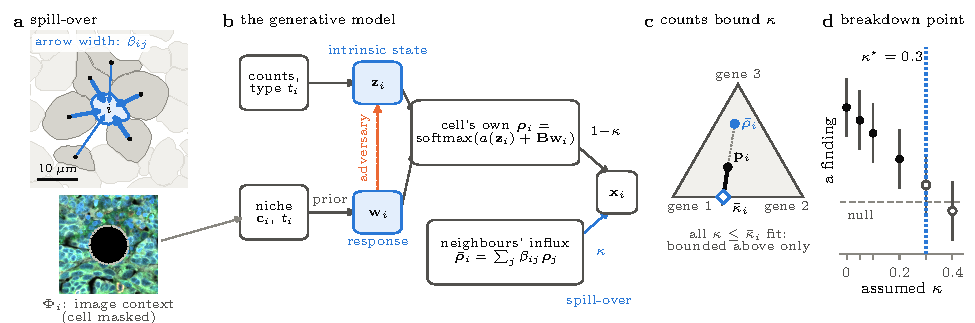
\includegraphics{recomb_fig1_overview}
\caption{DISCELL in four panels. \textbf{a},~Spill-over on segmented cells of the primary section: a cell (blue) receives transcripts from its first ring in proportion to the kernel weights $\beta_{ij}$ (arrow widths). Below: the morphology image, embedded as $\vPhi_i$ into the niche descriptor $\vc_i$ (grey arrow), with a $25\um$ disc around the cell masked out. \textbf{b},~The generative model (\cref{sec:generative}): $\vz_i$ and $\vw_i$, whose prior is set by the niche and the type, decode to the cell's own composition $\vrho_i$, mixed with the neighbours' compositions at the fixed fraction $\kappa$; an adversary keeps the niche out of $\vz_i$ given the type. \textbf{c},~Why $\kappa$ is swept (\cref{prop:kappa-bound}): on the simplex of three genes, each assumed $\kappa$ implies a clean composition on a line from the observed $\vp_i$ away from the influx $\rhobar_i$; every $\kappa$ fits until a gene's share would turn negative at $\bar\kappa_i$. \textbf{d},~The breakdown point (\cref{def:breakdown}): $\kappa^\star$ is the smallest grid value at which a finding's interval reaches its null value. b--d are schematic.}
\label{fig:overview}
\end{figure*}

\subsection{Generative model}
\label{sec:generative}
\label{sec:setting}

For each of $N$ segmented cells $i$ on one section we observe a count vector $\vx_i$ over $G$ genes with total $\ell_i$, a lineage label $t_i \in \{1,\dots,K\}$, its position and the morphology image around it. Two cells are neighbours if their Voronoi cells share a face (Delaunay adjacency), with edges longer than $40\um$ pruned; $\nbr{i}$ is the neighbour set of $i$. The model is
\begin{align}
  \vz_i &\sim \N(\mathbf{0}, \vI), \label{eq:gen-z}\\
  \vw_i \mid \vc_i, t_i &\sim \N\big(\mpsi(\vc_i, t_i),\, \sigma_w^2 \vI\big), \label{eq:gen-w}\\
  \vrho_i &= \softmax\big(\underbrace{a(\vz_i)}_{\text{intrinsic}} + \underbrace{\vB\vw_i}_{\text{response}}\big), \label{eq:gen-rho}\\
  \rhobar_i &= \textstyle\sum_{j \in \nbr{i}} \beta_{ij}\, \vrho_j, \label{eq:gen-rhobar}\\
  \vp_i &= (1-\kappa)\, \vrho_i + \underbrace{\kappa\, \rhobar_i}_{\text{spill-over}}, \label{eq:gen-p}\\
  \vx_i \mid \ell_i &\sim \Mult(\ell_i, \vp_i). \label{eq:gen-x}
\end{align}
Here $\vrho_i$ is the cell's own, \emph{clean} composition over genes. Its intrinsic part decodes $\vz_i \in \R^{\dz}$; its response part is linear in $\vw_i \in \R^{\dw}$, so that column $k$ of the loadings $\vB$ is a gene programme and $w_{ik}$ is how far the cell has moved along it. The decoder has no type input: the only route from identity to expression runs through $\vz_i$, which therefore carries the type together with what the label discretises away, such as cell-cycle phase. The prior mean $\mpsi(\vc_i, t_i)$ is the response expected of a cell of type $t_i$ in niche $\vc_i$; the prior scale is fixed at $\sigma_w = 1$, which pins the scale of $\vw$ against that of $\vB$.

\paragraph{The niche descriptor.}
$\vc_i$ is a deterministic function of the data, shared by co-located cells and containing no latent:
\begin{equation}
  \vc_i = \GAT\big(\embed(t_i);\ \{t_j\}_{j \in \nbr{i}}\big) \oplus \vPhi_i \oplus \mathbf{1}[\nbr{i} {=} \emptyset].
  \label{eq:context-gat}
\end{equation}
The first part is one graph-attention layer \citep{brody2022} over the neighbours' types, queried with the cell's own type, which amounts to a learned, type-specific reweighting of the neighbour-type composition $\vy_i$. The second, $\vPhi_i$, is the embedding by a frozen pretrained image model \citep{kronos2025} of a $128\um$ morphology crop around the cell, in which a disc of radius $25\um$ around the cell is set to zero, so that it describes the surrounding tissue and not the cell. No distances enter, so that the attention cannot rediscover the spill-over kernel and merge the two mechanisms the model separates (\suppref{app:graph}).

\paragraph{Spill-over.}
The influx $\rhobar_i$ is the neighbours' clean compositions averaged with a fixed kernel, $\beta_{ij} \propto f_{ij}\exp(-d_{ij}/\tau)$, normalised over $\nbr{i}$, where $d_{ij}$ is the distance between centroids, $f_{ij}$ the length of the shared Voronoi face and $\tau = 20\um$. The kernel is computed once and not learned, unlike resolVI's per-cell weights. The spill-over it represents has a specific form: one hop, one fraction for the whole section, and no gene dependence; an isolated cell receives none (\suppref{app:bound}).

\subsection{Inference and objective}
\label{sec:inference}
\label{sec:objective}
\label{sec:batching}

Both latents have amortised diagonal-Gaussian posteriors. The encoder of $q(\vz_i \mid \vx_i, t_i)$ reads the cell's normalised log counts, its log total and its type, never the niche; $q(\vw_i \mid \vc_i, t_i, \vz_i, \vx_i)$ reads the niche and the cell. Writing $r_i(\vw) = \ell_i^{-1}\sum_g x_{ig}\log p_{ig}(\vz_i, \vw)$ for the reconstruction per count, the training objective, maximised, is
\begin{equation}
\begin{split}
  J = \tfrac{1}{|\mathcal{S}|}\textstyle\sum_{i \in \mathcal{S}} \Big[\,& r_i(\vw_i) + \omega\, r_i(\wbreve_i) - \alphaa \Adv_i \\
  & - (1+\omega)\,\alphaz \KL\big(q(\vz_i) \,\|\, p(\vz_i)\big) \\
  & - \alphaw \KL\big(q(\vw_i) \,\|\, p(\vw_i \mid \vc_i, t_i)\big) \Big],
\end{split}
\label{eq:objective}
\end{equation}
over a batch $\mathcal{S}$ of cells. With $\omega = 0$ and $\alphaa = 0$ this is an evidence lower bound, scaled by depth so that the weights transfer between sections of different depth. The second term is the \emph{intrinsic path}: the same decoder evaluated with $\wbreve_i$ drawn from the prior instead of the posterior, a second bound on the same evidence \citep{slavutsky2025} that asks $\vz_i$ to explain the cell given only the response \emph{expected} in its niche. It keeps the type out of $\vw$: refitted with $\omega = 0$, the response's agreement with type rises on all four sections (\suppref{app:sensitivity}). The last term is the adversary of \cref{sec:invariance}. The neighbours' $\vrho_j$ enter $\rhobar_i$ under a stop-gradient, as in resolVI, and batches are contiguous spatial tiles with a two-hop halo (\suppref{app:tiles}). We use $\dz = 20$, $\dw = 6$, $\omega = 1$, $\alphaz = \tfrac12/\lbar$ with $\lbar$ the section's median total, and $\alphaw = 0.1$; the remaining settings are in \suppref{app:architecture}.

\subsection{Conditional invariance}
\label{sec:invariance}

The architecture keeps the niche out of the encoder of $\vz$, but not out of the counts it reads. The target is that, within a type, the intrinsic state says nothing about the niche:
\begin{equation}
  \I\big(\vz_i;\, [\vy_i, \vPhi_i] \mid t_i\big) = 0.
  \label{eq:invariance-target}
\end{equation}
It is conditional on the type because cell types cluster in space: an intrinsic state blind to the niche unconditionally would have to discard its type \citep{zhao2019inherent}. It covers the image too, so that a niche defined by morphology alone cannot hide in $\vz$. Two heads with parameters $\xi$ predict, from the posterior mean $\vmu_{z,i}$ and the type, the neighbour-type composition $\vy_i$ and a soft membership $\ephi_i$ of $\vPhi_i$ in $K$ image niches; the encoder is penalised by their skill beyond knowing the type alone,
\begin{equation}
\begin{split}
  \Adv_i = \;&\lambda_y\big[\CE(\vy_i, \ybar(t_i)) - \CE(\vy_i, \hat{\vy}_\xi(\vmu_{z,i}, t_i))\big] \\
  +\;&\CE(\ephi_i, \Phibar(t_i)) - \CE(\ephi_i, \hat{e}^{\Phi}_\xi(\vmu_{z,i}, t_i)),
\end{split}
\label{eq:adv}
\end{equation}
where $\ybar(t)$ and $\Phibar(t)$ are the mean targets of type $t$ and $\lambda_y = 3$ weights the composition, the channel of the spill-over confound. The heads maximise $\Adv_i$ with their own optimiser, the encoder minimises it, and it is zero at the optimum. Type-conditional adversarial invariance of an intrinsic latent against neighbour-type composition was introduced by MintFlow's per-type critics \citep{akbarnejad2025mintflow}; what we add is the image target and an independent test of the result.

\paragraph{The held-out probe.}
\label{sec:selection}
A training adversary that is defeated proves nothing \citep{elazar2018}, so invariance is graded by a \emph{fresh} predictor of each target block $b$ (the composition, and the leading principal components of $\vPhi$) from $(\vmu_{z,i}, t_i)$, trained on spatially separate training tiles and scored on held-out tiles. Its held-out gain over the type mean $\bar v_k(t)$, per component $k$ of the block,
\begin{equation}
  G_b = \frac{1}{|b|}\sum_{k \in b} \frac{1}{2}\log \frac{\E\big(v_k - \bar v_k(t)\big)^2}{\E\big(v_k - \hat v_k(\vmu_z, t)\big)^2},
  \label{eq:probe}
\end{equation}
estimates the predictive information from $\vz$ to the block given the type \citep{xu2020vinfo}. Its value with $\vmu_z$ permuted among cells of the same type is the chance floor. The \textbf{residual niche signal} is the excess of $G_b$ over that floor, reported as $1 - e^{-2\,\text{excess}}$: the share of the block's within-type variance that the probe explains beyond chance. We fit a linear (ridge) and a nonlinear (small perceptron) probe, each against its own floor, and compare with a fit without the adversary ($\alphaa = 0$). A probe at its floor bounds the dependence it can detect; it does not certify independence. Checkpoints are selected on held-out reconstruction while the agreement of $\vz$ with type (normalised mutual information of a $k$-means clustering of $\vmu_z$ with $t$) stays within $90\%$ of its running maximum (\suppref{app:architecture}).

\subsection{What is identified}
\label{sec:sweep}

Spill-over and response both make a cell resemble its neighbours, and a flexible model can fit either. The counts constrain the spill-over fraction in one direction only. Removing more and more of the neighbours' profile from a cell eventually drives some gene's share below zero, which no clean profile can have: this bounds $\kappa$ from above. Every smaller $\kappa$ yields a valid clean profile that reproduces the data exactly, so there is no lower bound (\cref{fig:overview}c).

\begin{proposition}\label{prop:kappa-bound}
Hold the neighbours' clean compositions, and hence $\rhobar_i$, fixed, and let $\vp_i = (1-\kappa)\vrho_i + \kappa\rhobar_i$ with $\vrho_i$ in the simplex. A fraction $\kappa' \in [0, 1)$ reproduces $\vp_i$ with a clean composition in the simplex if and only if $\kappa' \le \bar\kappa_i = \min_{g:\,\bar\rho_{ig} > 0} p_{ig}/\bar\rho_{ig}$. The true $\kappa$ satisfies $\kappa \le \bar\kappa_i$, with equality if and only if $\rho_{ig} = 0$ for some gene $g$ with $\bar\rho_{ig} > 0$.
\end{proposition}

\noindent The proof is in \suppref{app:kappa}. Even with the neighbours' clean profiles known, then, the counts bound $\kappa$ only from above, and pin it only through a gene that the cell cannot express itself. With finite counts the bound is soft; we do not compute it on our sections, and in simulation the fit offers no handle on $\kappa$ (\cref{sec:simulation}). Given $\kappa$, the response is identified at most up to a rotation of its programmes (as in factor analysis, its axes can be rotated, with the loadings counter-rotated, without changing the fit) and a per-type offset, so we report only rotation-invariant summaries and within-type contrasts (\suppref{app:symmetries}).

\paragraph{The sweep.}
We therefore do not estimate $\kappa$. We fit the model independently at each $\kappa \in \{0, 0.05, 0.1, 0.2, 0.3, 0.4\}$, with three seeds per value and every other weight held fixed, and check the held-out probe at each value, so that a change in a readout is not a change in the invariance. This is a sensitivity analysis with $\kappa$ as the sensitivity parameter, in the tradition of tipping-point and E-value analyses of unmeasured confounding \citep{rosenbaum2002,vanderweele2017}: the fractions compatible with the data form an interval from zero \citep{manski2003}, and the question asked of each finding is how far into it the finding survives.

\begin{definition}[Breakdown point]\label{def:breakdown}
For a signed contrast $r$, let $I_\kappa(r)$ be the interval of its mean over seeds at spill-over fraction $\kappa$. The contrast holds at $\kappa$ if $I_\kappa(r)$ excludes zero and every seed keeps the sign the contrast has at $\kappa = 0$. Its \emph{breakdown point} $\kappa^\star(r)$ is the smallest grid value at which it does not hold. If it does not hold at $\kappa = 0$, $r$ is no finding; if it holds at every grid value, $\kappa^\star(r)$ is reported as exceeding the top of the grid.
\end{definition}

\noindent The interval comes from a spatial block bootstrap over tiles, Bonferroni-adjusted over the contrasts claimed on a section. A finding with $\kappa^\star > 0.4$ cannot be explained by spill-over of the modelled form up to four times the typical misassignment of about a tenth of a cell's transcripts \citep{yang2025mistic}; spill-over of another form (longer-ranged, gene-specific, depth-dependent) is not ruled out. Readouts shrink with $\kappa$ by construction, so only sign and interval are read. A contrast without a sign at $\kappa = 0$, because it is zero there by construction or measures decoding rather than spill-over removal, is shown as a trajectory instead (\suppref{app:sweep}). Nothing in the protocol is specific to DISCELL: any model with a spill-over term at a fixed fraction can attach a breakdown point to any spatial readout.


\section{Experiments}
\label{sec:experiments}
\subsection{Setup}
\label{sec:setup}
% 03_1_setup.tex -- budget 0.4 p. Sections, labels, splits and seeds, baselines + fairness, kappa = 0.1.

\paragraph{Sections and labels.}
We fit DISCELL to four sections from one imaging-based assay with a panel of about five thousand genes \citep{janesick2023}: ovarian cancer fixed in formalin and embedded in paraffin (FFPE), our primary section \citep{tenx_ovarian_ffpe}; lung cancer, FFPE \citep{tenx_lung_ffpe}; fresh-frozen (FF) ovarian cancer, with about eight times the counts per cell \citep{tenx_ovary_ff}; and one core of a paediatric lung tissue microarray (TMA) \citep{williamskatek2026fishing}. They hold $69{,}000$ to $1.16$ million cells (\suppref{app:sections}). A serial section of the TMA core, on a second slide, is never fitted; it is read only through the models fitted to the core. Cells carry lineage labels (curated on the ovarian FFPE section and the TMA, marker-annotated clusters elsewhere), in which finer states and locations are merged into their lineage; unlabelled cells train as their own class and are never scored.

\paragraph{Splits, seeds and the operating point.}
$15\%$ of each section's contiguous spatial tiles are held out, and every readout is taken on held-out cells. Every configuration is fitted with three seeds, each redrawing the split, and reported as the mean with the range over seeds. One configuration, with $\alphaz$ scaled to depth, serves every section. Single fits are read at $\kappa = 0.1$, the typical misassignment \citep{yang2025mistic}. This is an operating point, not an estimate: every finding below is re-examined across the sweep in \cref{sec:robustness}.

\paragraph{Comparison methods and fairness.}
We compare with resolVI \citep{ergen2026resolvi}, a single-latent model of spill-over, and with SIMVI \citep{dong2025simvi}, MintFlow \citep{akbarnejad2025mintflow} and Cellina \citep{moeed2026cellina}, which split each cell into an intrinsic and a context latent. All are scored by the same readouts of their intrinsic latent on our held-out cells. The comparison is asymmetric in two opposite directions: DISCELL's weights were calibrated on these sections (\suppref{app:sensitivity}), while the comparison methods ran at their published defaults and were trained, as their software is designed, on all cells, our held-out cells included. Cellina removes a spatial-domain label from its intrinsic latent; our sections have none, so it is also shown with our niche label as its domain, its best case on our probe.

\subsection{Simulation}
\label{sec:simulation}
% 03_2_simulation.tex -- budget 0.5 p. C7; the planted spill-over control lives in 3.7 only.

We simulate sections from the generative model of \cref{sec:generative}: $6{,}000$ cells of eight spatially clustered types, a response linear in the neighbour composition, and spill-over planted at $\kappa = 0$ or $0.2$, three worlds each, each fitted with three seeds (\suppref{app:synthetic}, \cref{tab:synthetic}).

\paragraph{Recovery, and what the adversary does.}
The intrinsic state agrees with the planted type (NMI $0.80$ to $0.96$), as well as clusters of the counts or better in $17$ of $18$ fits; the response correlates with the planted one (first canonical correlation $0.83$ to $0.95$); the loadings span the planted programmes better than random subspaces in every fit; and $\vz$ carries almost none of the planted niche (within-type $R^2$ of composition at most $0.04$). Without the adversary, the response correlates at only $0.29$ to $0.91$ and the niche moves into $\vz$ ($R^2$ $0.11$ to $0.19$).

\paragraph{A wrong $\kappa$ costs little, so the fit cannot find the right one.}
On the worlds planted at $\kappa = 0.2$, fits at any assumed $\kappa$ from $0$ to $0.4$ recover the planted quantities about equally well (\cref{fig:synthetic-misspec}). Recovery does not hinge on guessing $\kappa$, and offers no handle on it: the non-identifiability of \cref{prop:kappa-bound}, seen in practice. The encoder's posterior mean is measurably off the exact one, more so at the final configuration than in development (\suppref{app:planted}). A positive control for the breakdown point, with spill-over planted at a known fraction, is in \cref{sec:robustness}.

\subsection{What the Intrinsic State and the Response Carry}
\label{sec:intrinsic-response}
\label{sec:results-z}
\label{sec:results-w}
% 03_3_intrinsic_and_response.tex -- budget 1.2 p. Claims C3, C4.

\begin{figure}[t]
\centering
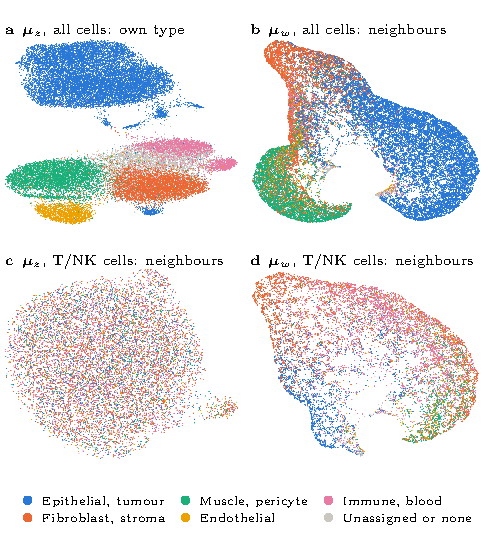
\includegraphics[width=\columnwidth]{fig_latents_main}
\caption{The two latents on the ovarian FFPE section (one seed; UMAP of the posterior means). \textbf{a},~$\vmu_z$ of $30{,}000$ random cells, coloured by the cell's own lineage. \textbf{b},~$\vmu_w$ of the same cells, coloured by the lineage that dominates the cell's neighbours. \textbf{c},~$\vmu_z$ of T/NK cells, the large type with the most mixed neighbourhoods (chosen by that rule), coloured by their neighbours. \textbf{d},~$\vmu_w$ of the same T/NK cells. UMAP can exaggerate separation; the held-out probe measures what c and d show.}
\label{fig:latents-main}
\end{figure}

\Cref{fig:latents-main} shows the split at a glance: $\vz$ groups cells by their own lineage (a), $\vw$ by their neighbours' (b), and within the T/NK cells $\vz$ shows no grouping by the neighbours (c) while $\vw$ is ordered by them (d). \Cref{tab:headline-main} measures this on every section.

\input{\tablesdir/headline_main}

\paragraph{The intrinsic state keeps the type and the cell cycle.}
On every section $\vz$ agrees with the lineage labels (NMI $0.62$ to $0.74$) and carries the cell cycle, a within-type state the labels do not encode: on the most strongly cycling tenth of held-out cells, $\vz$ explains $19$ to $76\%$ of the variance of the cycle scores and $\vw$ at most $1\%$ (\cref{tab:headline-main}). The cycle score is a proxy computed from the same segmented counts, which spill-over from cycling neighbours also raises; the asymmetry shows where the model puts this axis, not that the score is free of spill-over. Read without refitting, the serial section gives what the core gives (NMI $0.61$ against $0.62$; cycle $R^2$ of $\vz$ $0.49$ against $0.50$): an out-of-sample replication on a second slide.

\paragraph{The adversary removes most of the niche from $\vz$.}
On the four fitted sections it cuts the residual niche signal (\cref{sec:invariance}) that a held-out linear probe finds in $\vz$ by $80$ to $93\%$. A nonlinear probe still finds $3.5$ to $5.5\%$ of the within-type variance of neighbour composition on every section (\cref{tab:probe}); on the TMA sections, which carry little niche signal even without the adversary, that is more than half of the original amount. A probe-free read agrees: the within-type spatial autocorrelation (Moran's I) of $\vz$ falls by $25$ to $48\%$ (\cref{fig:programmes}d).

\paragraph{The response carries the niche.}
$\vw$ holds $0.47$ to $0.60$ nats of information about the niche beyond a within-type permutation floor (\cref{tab:headline-main}), $85$ to $90\%$ of what the two latents carry together (\suppref{app:response}). Without the adversary the response nearly vanishes within types and $\vz$ takes up the niche instead (\suppref{app:moran}): on tissue, as in simulation, the adversary is what makes the split exist.

\paragraph{Held-out sublabels split as designed.}
The lineage labels merge finer curated classes that the model never saw: a tumour \emph{state} should go to $\vz$, a \emph{location} to $\vw$. On the primary section, held-out probes show a double dissociation (\suppref{app:subtype}). Tumour- against stroma-associated fibroblasts are read from $\vw$ with balanced accuracy $0.95$ (from $\vz$: $0.66$), and the same split of endothelial cells with $0.90$ ($0.67$). The four tumour states are read from $\vz$ with $0.79$ (from $\vw$: $0.41$; chance $0.25$). By the call fixed in advance, the proliferative and inflammatory states go to $\vz$ on all three seeds and the locations to $\vw$ on two of three. The exceptions are states that are also places: hypoxic VEGFA$^+$ tumour cells are read from both latents, and myofibroblasts on the TMA core better from $\vw$. Merging such a state into its lineage moves part of it into the response.

\paragraph{At the operating point the response is type-level.}
A held-out classifier separates tumour- from stroma-associated fibroblasts almost as well from the response's context prediction $\mpsi(\vc_i, t_i)$ alone as from the response itself (balanced accuracy $0.94$ against $0.95$; chance $0.5$), the posterior adds one part in a thousand or less to held-out reconstruction (\suppref{app:recon-modes}), and a per-cell response planted in simulation, twice the niche effect, is not detected (\suppref{app:planted-percell}). At $\alphaw = 0.1$ the response thus describes how a cell \emph{type} shifts with its niche, not how one cell deviates from that shift; the lung section is a partial exception.

\subsection{What the Response Encodes}
\label{sec:programmes}
% 03_4_programmes.tex -- budget 0.8 p. Claim C4b. Every value from data/datasets/<ds>/runs/finalL_s{0,1,2}/atlas
% and the validation files, via figures/src/recomb_fig_programmes.py (verification log in _reports/exp_a.md).

\begin{figure*}[t]
\centering
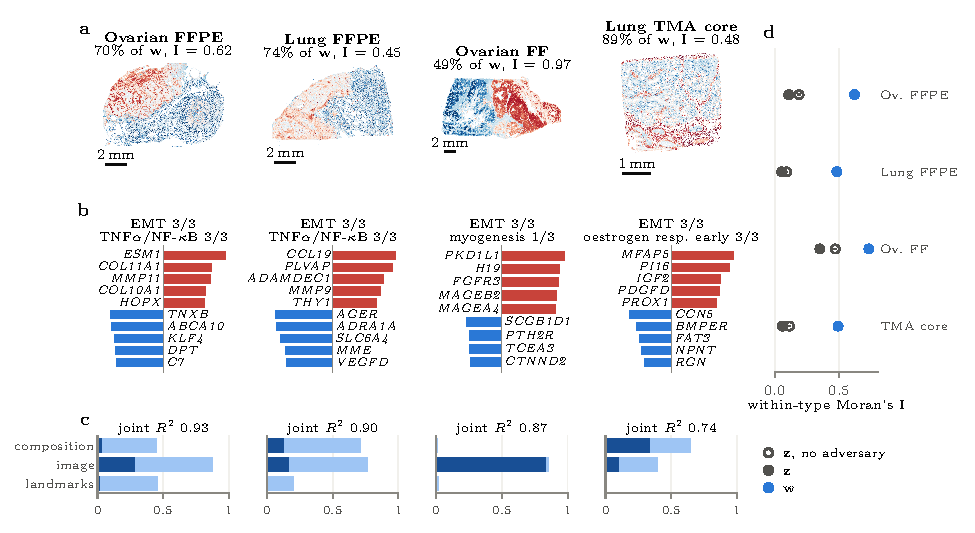
\includegraphics[width=\textwidth]{recomb_fig_programmes}
\caption{The leading response programme of each section, in one fit. \textbf{a},~Territory: each cell's shift toward the red (blue) genes of b, relative to its type's average (FF rotated), with the programme's share of $\vw$'s within-type variance and its within-type Moran's I. \textbf{b},~Signature: the five largest positive and negative gene loadings, scaled, and its two most significant hallmark labels \citep{liberzon2015hallmark}, with the number of seeds in which the matching programme carries each among its top three at $q \leq 0.05$. \textbf{c},~Drivers: cross-validated $R^2$ of the score from neighbour composition, image context and distances to landmarks (vessels, smooth muscle, the tumour--stroma interface, where annotated): alone (light), unique given the others (dark), all three together (title). \textbf{d},~Within-type Moran's I of $\vz$ without the adversary (two seeds), and of $\vz$ and $\vw$ in the final fits (three seeds): mean and range.}
\label{fig:programmes}
\end{figure*}

Within types, the response's variation lies in two or three programmes (four or five on the FF section, depending on the seed). Programmes, directions of $\vw$ read in gene space through $\vB$, are identified only up to rotation (\cref{sec:sweep}), so we describe each section's leading programme within one fit (\cref{fig:programmes}) and compare seeds only on its leading genes and hallmark labels.

\paragraph{The response maps territories.}
Within types, Moran's I of $\vw$ is $0.48$ to $0.73$, against $0.05$ to $0.11$ for $\vz$ on three sections and $0.35$ on the FF section (\cref{fig:programmes}d).

\paragraph{Each leading programme has a recognisable signature.}
On the ovarian FFPE section the leading programme ($70\%$ of the response's within-type variance) sets \textit{COL11A1}, \textit{MMP11}, \textit{COL10A1} and \textit{INHBA}, genes of the cancer-associated fibroblasts of invasive tumours, ovarian cancer included \citep{kim2010multicancer,zhu2021adipose}, against \textit{C7} and \textit{DPT}, genes of non-activated stromal fibroblasts \citep{zhu2021adipose,buechler2021crosstissue}, \textit{TNXB} and inflammatory genes (\textit{IL6}, \textit{PTGS2}). Its territory lies around the tumour: in fibroblasts, macrophages, T/NK and endothelial cells the score rises with the share of tumour cells among the neighbours. The same genes lead it in all three seeds, as do its hallmark labels, epithelial--mesenchymal transition (EMT) and TNF$\alpha$/NF-$\kappa$B signalling. On the lung FFPE section the leading programme sets \textit{CCL19}, a gene of immune-interacting fibroblasts in inflamed tissue \citep{korsunsky2022stromal}, with \textit{PLVAP}, \textit{ADAMDEC1} and \textit{MMP9} against the alveolar \textit{AGER} and \textit{MME}, with the same two labels in all seeds; on the TMA core, the adventitial-fibroblast genes \textit{MFAP5} and \textit{PI16}, with \textit{PDGFD}, against the alveolar-fibroblast gene \textit{NPNT}, with \textit{CCN5} and \textit{FAT3} \citep{tsukui2020collagen,hanley2023lungcaf}. The labels are coarse: EMT, dominated by extracellular-matrix genes, is significant on most programmes (\cref{fig:hallmarks}), so the genes are the more specific read.

\paragraph{What drives each programme.}
As the response is close to its prior mean, composition and image together explain most of each programme (joint $R^2$ $0.74$ to $0.93$, \cref{fig:programmes}c). The image carries the unique share on the ovarian FFPE section, composition on the TMA core, both on the lung section. Distances to landmarks, not a model input, explain up to $0.46$ of the ovarian programme alone but at most $0.02$ beyond composition and image, which already reflect them.

\paragraph{The FF section is the least stable.}
Its leading programme follows the image almost alone (unique $R^2$ $0.83$), splits the section into two large regions and is led by tumour-cell genes such as the cancer--testis antigens \textit{MAGEA4} and \textit{MAGEB2}: a regional difference between tumour areas explains it as well as a response does. Across seeds its leading direction matches least well (cosine as low as $0.67$, against $0.72$ to $0.98$ elsewhere), the number of programmes changes, and only its EMT label recurs. We do not interpret it as a niche response.

\subsection{Comparison with Other Methods}
\label{sec:comparison}
% 03_5_comparison.tex -- budget 1.1 p. Claims C2, C6.
% Freeze rule: C2 and C6 are worded finally only after the MintFlow refits land; every
%   MintFlow-dependent statement carries \pending{MintFlow refits}.

\begin{figure*}[t]
\centering
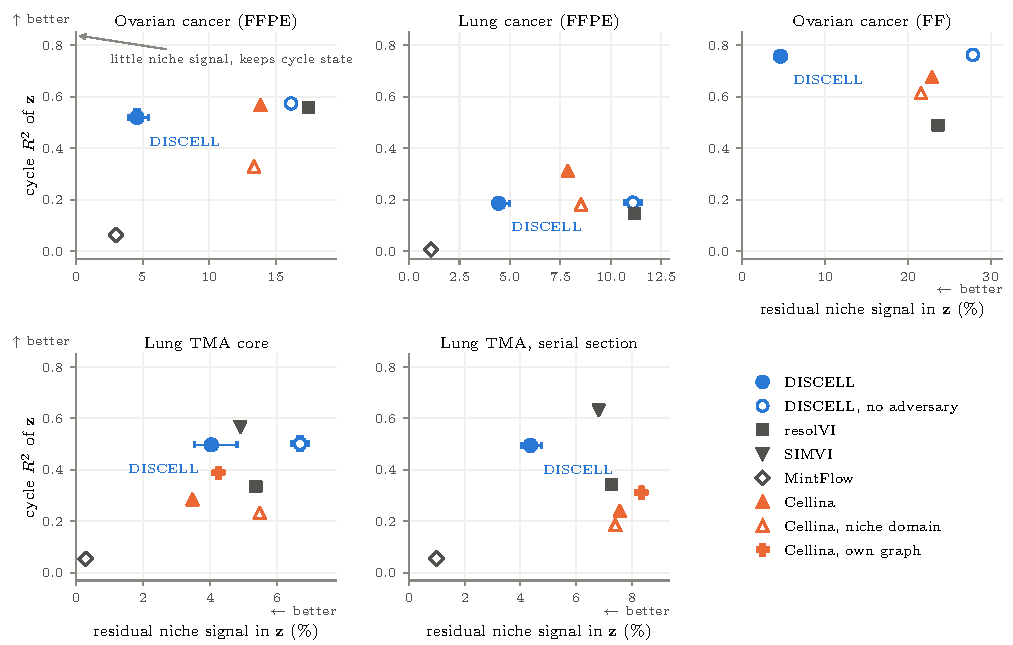
\includegraphics[width=\textwidth]{recomb_tradeoff}
\caption{Residual niche signal in the intrinsic latent against the cell-cycle state it keeps, per section. \emph{Horizontal}: residual niche signal (nonlinear probe, neighbour composition; \cref{sec:invariance}), in \%. \emph{Vertical}: cycle $R^2$ of the intrinsic latent, as in \cref{tab:headline-main}. The desirable corner is the top left. DISCELL: mean over three seeds, bars the range; open circle: DISCELL without the adversary. resolVI keeps a single latent and is shown as a reference. Cellina is also shown with our niche label as the domain its adversary removes (its best case on this probe), and on the TMA sections on its own neighbour graph. SIMVI ran out of memory on a 24\,GB GPU on the three larger sections, and MintFlow could not be fitted on the FF section. Values: \cref{tab:probe,tab:battery}. \pending{MintFlow refits: MintFlow's points are redrawn from the new fits}}
\label{fig:tradeoff}
\end{figure*}

\Cref{fig:tradeoff} sets two reads of each method's intrinsic latent against each other: the residual niche signal and the within-type cell-cycle state the latent keeps. Cycle state is the one read of retained state that needs no label and varies within a type; it was fixed for all methods after earlier baseline reads but before the final scoring. Agreement with the type label (NMI) rewards label fidelity, which MintFlow and Cellina are trained towards, and on it both score above DISCELL (\cref{tab:battery}).

No method both carries less residual niche signal than DISCELL and keeps more cycle state, on any section. Under a linear probe, DISCELL's intrinsic state carries the least neighbour composition and the least image information of all methods on every section (on ovarian FFPE, $1.0$--$1.1\%$ of the within-type variance of composition, against $4.0\%$ for MintFlow, the next lowest). Under the nonlinear probe of \cref{fig:tradeoff}, only MintFlow carries less wherever it ran, and its intrinsic latent keeps almost no within-type state (cycle $R^2 \le 0.06$); on the TMA core, Cellina's residual is at DISCELL's lowest seed, with less cycle state. Methods that keep more cycle state carry more residual signal, and on the FF section DISCELL is best on both axes. DISCELL's latent is also the one least predicted by the niche: its mirror $R^2$ (\cref{tab:headline-main}), computed for every method from DISCELL's niche descriptor, is the lowest on four of the five sections, MintFlow being lower on the serial one. \pending{MintFlow refits: the MintFlow comparisons in this paragraph are re-scored}

resolVI keeps a single latent, so it is a reference for a model that does not separate the niche, not a competitor here; its residual is two to five times DISCELL's on the three whole-slide sections. Nor is the result reproduced by adding an adversary to another model. Given our niche label as the domain its adversary removes, Cellina's best case on this probe, its residual does not consistently fall, and it loses agreement with type and cycle state on every section; on its own neighbour graph it keeps less cycle state than DISCELL at a similar or higher residual (\suppref{app:baselines}). The separation comes from the architecture, not from the adversary alone.

Held-out reconstruction is within $0.015$ nats per count of the best method on every section and best on the two whole-slide FFPE sections (\cref{tab:battery}). One DISCELL fit, its evaluations included, is up to $2.6$ times faster than the fastest comparison method, Cellina, on three of the four sections and slower than it on the FF section; it is over a hundred times faster than MintFlow wherever MintFlow could be run (\cref{tab:timing}). The honest unit is the sweep of $18$ fits (\cref{sec:sweep}): at the operating point's run time it takes at most $2.8$ hours on each section where MintFlow ran, less than one MintFlow fit there ($9$ to $16$ hours), and on the TMA core less than one SIMVI fit; on the FF section it takes longer than one resolVI fit. \pending{MintFlow refits: MintFlow's reconstruction and run times}

\subsection{Relocation}
\label{sec:relocation}
% 03_6_relocation.tex -- budget 0.8 p. Claim C5.
% tab:relocation is a hand table: every number is traced from
%   ../aistats/tables/generated/cellina_cf.tex (tab:cellina-cf, DISCELL's first seed beside Cellina).

\begin{table}[t]
\centering
\caption{Relocation, DISCELL against Cellina's neighbour-rewiring counterfactual, on the same panels, niches and ceilings (DISCELL's first seed, which supplies the panels; Cellina refitted on the training tiles). \emph{Ceiling}: share of the reproducible between-niche difference recovered, over the panels whose ceiling can be read. \emph{Single cell}: share of the distribution gap to the target niche's own cells that the moved cells close. \emph{Twin}: how much closer, in expression, each target cell lies to the moved cell nearest it in intrinsic state than to a random moved cell. D: DISCELL; C: Cellina. Higher is better; bold marks the better of the two. $^{a}$A single readable panel. Intervals: \cref{tab:cellina-cf}.}
\label{tab:relocation}
\footnotesize
\setlength{\tabcolsep}{2.8pt}
\begin{tabular}{@{}lcccccc@{}}
\toprule
 & \multicolumn{2}{c}{Ceiling} & \multicolumn{2}{c}{Single cell} & \multicolumn{2}{c}{Twin} \\
\cmidrule(lr){2-3}\cmidrule(lr){4-5}\cmidrule(lr){6-7}
Section & D & C & D & C & D & C \\
\midrule
Ovarian FFPE & 0.650 & \textbf{0.731} & \textbf{0.789} & 0.681 & \textbf{0.398} & 0.361 \\
Lung FFPE    & \textbf{0.743} & 0.703 & \textbf{0.826} & 0.757 & 0.432 & \textbf{0.435} \\
Ovarian FF   & \textbf{0.677} & 0.566 & \textbf{0.823} & 0.602 & \textbf{0.437} & 0.330 \\
TMA core     & 0.711 & \textbf{0.899}$^{a}$ & \textbf{0.814} & 0.801 & \textbf{0.464} & 0.284 \\
\bottomrule
\end{tabular}
\end{table}

\emph{Relocation} asks how a cell type's expression would change if its cells sat in another niche. DISCELL answers it by keeping each cell's intrinsic state, moving the prior of its response and its spill-over influx to the target niche, and decoding. For each type and pair of niches (a panel), the predicted change in the type's mean expression is scored against the observed difference between the two niches, as a share of the part of that difference that is reproducible between two random halves of the cells (the noise ceiling); only panels whose ceiling is high enough to be read count (\suppref{app:readouts}).

Moved to another niche, a cell type's predicted shift recovers $0.65$ to $0.73$ of the reproducible between-niche difference (\cref{tab:headline-full}). The response programmes of \cref{sec:programmes} carry most of it: predicted from the programmes alone, the shift recovers $0.52$ to $0.64$ of the ceiling, and from the spill-over alone $0.21$ to $0.39$ (the two parts are not additive; \cref{tab:cellina-cf}).

Cellina \citep{moeed2026cellina} also predicts expression under a rewired neighbourhood, so we score its counterfactual by the same reads on the same panels (\cref{tab:relocation}). The comparison is mixed. DISCELL's moved cells are closer to the target cells' own distribution on every section, with disjoint intervals on three, and DISCELL leads on all three reads on the FF section. Cellina recovers more of the ceiling on the ovarian FFPE section, and on the TMA core on its single readable panel, and is narrowly ahead on the twin read on lung. Most scored cells lie in the model's training tiles; scored on held-out tiles only, DISCELL's share of the ceiling moves in both directions across fits, so it shows no systematic in-sample advantage, while Cellina's falls on both FFPE sections, on lung from $0.70$ to $0.49$, below DISCELL's range (\cref{tab:transport-heldout}).

Would a plain regression do as well? Regressing each type's expression shift directly on neighbour composition, from the counts as observed, recovers \pending{plain-regression reference} of the ceiling.
% Planned follow-up sentence, one of: below DISCELL -> modelling spill-over and the intrinsic state adds
%   accuracy beyond what niche composition predicts; level -> DISCELL's advantage lies in the separation
%   (an intrinsic state largely free of the niche, spill-over modelled), not in relocation accuracy.

\subsection{Robustness to Spill-over}
\label{sec:robustness}
\label{sec:results-sweep}
% 03_7_robustness.tex -- budget 1.0 p. Claim C1.
% Freeze rule: C1 is worded finally only after the breakdown-gaps queue lands (~21:00).
% tab:kappa-star is generated (scripts/paper_tables.py --only breakdown_main); rerun it after the
%   breakdown-gaps queue lands, then recount the breaks below.

\input{\tablesdir/breakdown_main}

Every section was refitted along the sweep of \cref{sec:sweep}, and \cref{tab:kappa-star} gives each finding of \crefrange{sec:intrinsic-response}{sec:relocation} its breakdown point. The findings are split in two groups. The \emph{allocation checks}, that $\vz$ keeps the cycle and $\vw$ the niche, are favoured by the model's design; the \emph{biological claims} are the stronger test.

The test has teeth. It breaks three findings: the response's lean toward ligand--receptor genes on the FF section ($\kappa^\star = 0.2$), and the relocation's margin over its spill-over part on the ovarian and lung FFPE sections ($\kappa^\star = 0.4$ and $0.3$, where a seed changes sign). These are the findings that spill-over could most plausibly produce: a gene-specific spill-over would create the lean, and the margin measures what the prediction adds to spill-over. Every other finding holds across the whole grid on every section. \pending{breakdown gaps: recount} Two contrasts first in the graded set were moved to trajectories after reading, by the rule of \cref{sec:sweep}: one, between marker pairs, measures decoding, and the other, the relocation's margin over its programme part, is zero by construction at $\kappa = 0$.

A positive control shows that the rule detects spill-over when it is there. In simulation, we plant a spatial contrast created only by spill-over at a known fraction beside a genuine response contrast, and run the same sweep. The prediction, set before the run, is that the spill-over contrast breaks at the first grid point at or above the planted fraction, while the response contrast holds. \pending{planted spill-over control}
% If kappa* does not track the planted fraction: report it as found and present the breakdown point as a lower-power check.

Of the spill-over forms the sweep leaves open, several were refitted on the primary section, three seeds each (\suppref{app:sensitivity}): per-cell and per-gene spill-over rates move no read by more than $1.3$ seed standard deviations, but a fixed false-positive floor lowers the relocation read from $0.65$ to $0.50$.


\section{Discussion}
\label{sec:discussion}
% 04_discussion.tex -- budget 0.6 p. Each claim once, with its reference and why it matters;
% one limitations paragraph pointing to the supplement; then the code link.

Spill-over and a niche response compete for the same counts, and the counts cannot say how much of a cell's resemblance to its neighbours is which (\cref{prop:kappa-bound}). DISCELL therefore treats the spill-over fraction as a sensitivity parameter, not an estimate, and attaches a breakdown point to each finding. The test is not vacuous: it breaks the findings that spill-over could most plausibly produce and leaves the others standing across the grid (\cref{sec:robustness}). The protocol transfers to any model with a spill-over term, and lets a reader judge a spatial claim by how much misassignment it tolerates.

Separating the two mechanisms leaves an intrinsic state that keeps the cell type and the cell cycle and loses most of the niche, on a held-out serial section as on the fitted ones (\cref{sec:intrinsic-response}). Against four methods, none carries less niche signal while keeping more within-type state, and the separation is not reproduced by giving another model an adversary (\cref{sec:comparison}). For biology, the response is where the niche goes: it maps tissue territories with recognisable programmes (\cref{sec:programmes}), held-out locations are read from it while tumour states are read from the intrinsic state, and relocating a cell type predicts most of the reproducible shift between niches (\cref{sec:relocation}).

\paragraph{Limitations.}
The sweep rules out only spill-over of the modelled form, one hop, one fraction per section and no gene dependence; a fixed false-positive floor already moves the primary relocation read (\cref{sec:robustness}). All sections come from one platform. At the operating weights the response is type-level: it describes how a cell type shifts with its niche, not how one cell deviates from that shift (\cref{sec:intrinsic-response}). The cycle score that grades the intrinsic state is a proxy computed from the same segmented counts. DISCELL's weights were calibrated on these sections, while the comparison methods ran at their defaults (\cref{sec:setup}). The full list is in \suppref{app:limitations}.

\paragraph{Code.} \codelink.


\markmainend
% ---------------- bibliography (not counted) ----------------
\bibliographystyle{unsrtnat}
\bibliography{../aistats/references}
% the supplement follows the references in main.pdf (author, 2026-10-01); the
% separate supplement.pdf is still built for submission as supplementary material
\IfFileExists{supplement.pdf}{\clearpage\includepdf[pages=-]{supplement.pdf}}{}

\end{document}
